\documentclass[border=5pt]{standalone}
\usepackage[T1]{fontenc}
\usepackage{helvet}
\renewcommand{\familydefault}{\sfdefault}
\usepackage{tikz}
\usepackage{amsmath}
\usetikzlibrary{positioning, arrows.meta, shapes.geometric, calc, shadows, fit}

% Define colors
\definecolor{emeraldpine}{HTML}{1A4D3E}
\definecolor{harvardcrimson}{HTML}{A51C30}
\definecolor{ethdarkblue}{HTML}{1F407A}
\definecolor{ethpetrol}{HTML}{007A87}
\definecolor{ethbronze}{HTML}{B87333}
\definecolor{ink}{HTML}{1A202C}
\definecolor{softink}{HTML}{4A5568}
\definecolor{paleink}{HTML}{A0AEC0}
\definecolor{cardbg}{HTML}{F8FAFC}
\definecolor{shadecolor}{HTML}{F4F6F9}

\begin{document}
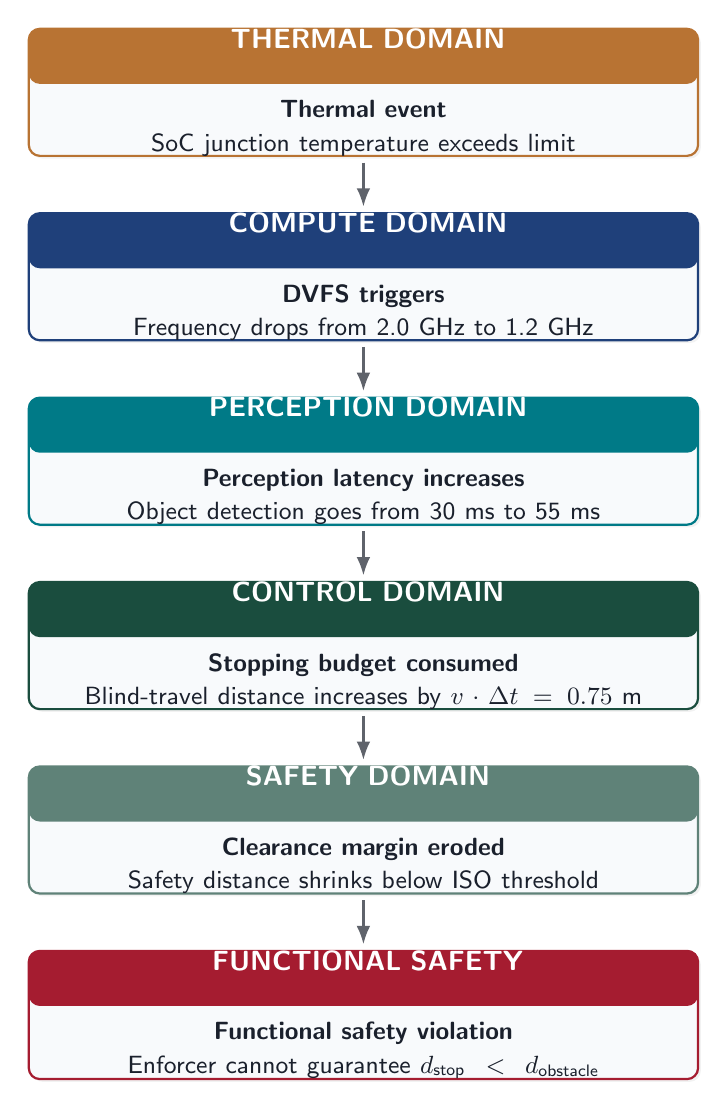
\begin{tikzpicture}[
    >=Latex,
    node distance=0.7cm,
    box/.style={
        rectangle,
        rounded corners=4pt,
        draw=#1,
        thick,
        fill=cardbg,
        text width=8.5cm,
        align=center,
        inner sep=0pt,
        drop shadow={opacity=0.1, shadow xshift=1pt, shadow yshift=-1pt},
        path picture={
            \fill[#1] (path picture bounding box.north west) rectangle ([yshift=-0.7cm]path picture bounding box.north east);
        }
    },
    arrow/.style={
        ->,
        thick,
        draw=ink!70,
        shorten >=2pt,
        shorten <=2pt
    }
]

% Define a macro for a node with header and content
\newcommand{\chainnode}[6]{
    % #1 = node name
    % #2 = color
    % #3 = header text
    % #4 = title text
    % #5 = subtitle text
    % #6 = placement (e.g., below=of previous)
    
    \node[box=#2, #6] (#1) {
        \vspace{0.15cm}
        \textcolor{white}{\textbf{#3}}\\[0.35cm]
        {\small\color{ink}\textbf{#4}\\
        #5}\\[0.25cm]
    };
}

% 1. Thermal Event
\chainnode{n1}{ethbronze}
  {THERMAL DOMAIN}
  {Thermal event}
  {SoC junction temperature exceeds limit}
  {}

% 2. Compute/DVFS
\chainnode{n2}{ethdarkblue}
  {COMPUTE DOMAIN}
  {DVFS triggers}
  {Frequency drops from 2.0 GHz to 1.2 GHz}
  {below=of n1}

% 3. Perception
\chainnode{n3}{ethpetrol}
  {PERCEPTION DOMAIN}
  {Perception latency increases}
  {Object detection goes from 30 ms to 55 ms}
  {below=of n2}

% 4. Control
\chainnode{n4}{emeraldpine}
  {CONTROL DOMAIN}
  {Stopping budget consumed}
  {Blind-travel distance increases by $v \cdot \Delta t = 0.75$ m}
  {below=of n3}

% 5. System Safety Margin
\chainnode{n5}{emeraldpine!70}
  {SAFETY DOMAIN}
  {Clearance margin eroded}
  {Safety distance shrinks below ISO threshold}
  {below=of n4}

% 6. Safety Violation
\chainnode{n6}{harvardcrimson}
  {FUNCTIONAL SAFETY}
  {Functional safety violation}
  {Enforcer cannot guarantee $d_{\text{stop}} < d_{\text{obstacle}}$}
  {below=of n5}

% Draw arrows
\draw[arrow] (n1) -- (n2);
\draw[arrow] (n2) -- (n3);
\draw[arrow] (n3) -- (n4);
\draw[arrow] (n4) -- (n5);
\draw[arrow] (n5) -- (n6);

\end{tikzpicture}
\end{document}
